\section{Shape Matching}
\label{sec:shape-matching}
The shape matching problem is to find a mapping between shapes.
For an illustration see Figure~\ref{fig:shape-matching}.
We follow the formulation of~\cite{windheuser2011geometrically,windheuser2011large} of the shape matching problem as an ILP for orientation preserving geometrically consistent matching.

\begin{figure}[h]
\centering
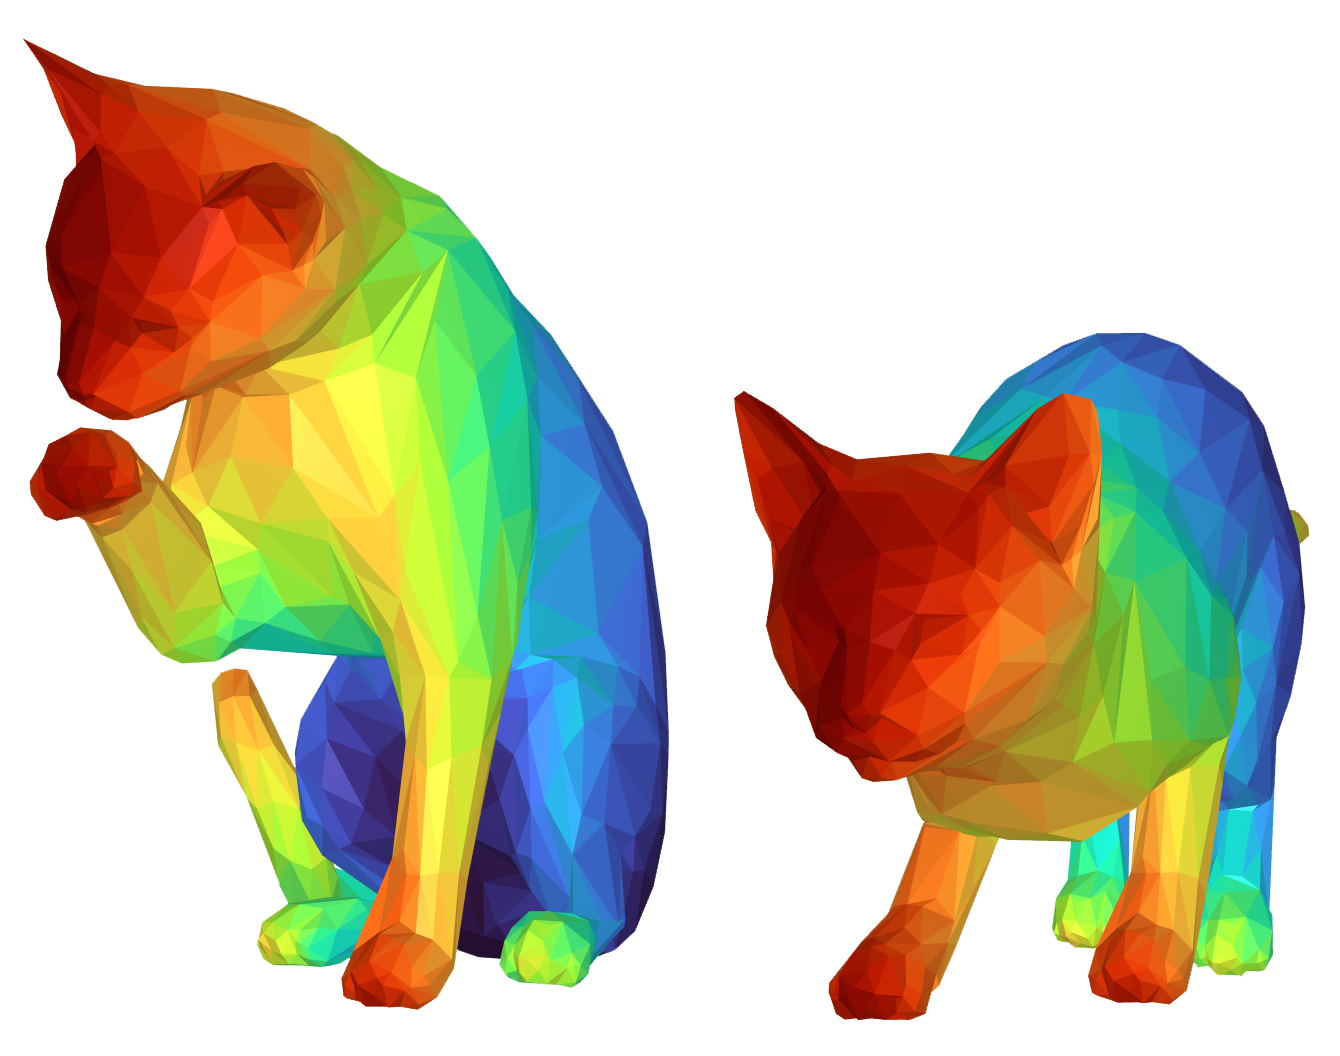
\includegraphics[width=0.8\columnwidth]{images/cat-matching}
\caption{Shape matching of a cat in different poses. Colors encode matches of triangles.}
\label{fig:shape-matching}
\end{figure}

\begin{definition}[Shape]
We define a shape $X$ as a triplet $(V_X, E_X,F_X)$ of vertices $V_X$, 
edges 
$E_X \subset V_X \times V_X$ 
and triangles 
$F_X \subset V_X \times V_X \times V_X$,
such that the manifold induced by the triangles is oriented and has no boundaries.

We denote by $\overline{F}_{\bullet}$ the space of all also possibly degenerated triangles, i.e.\ edges and vertices as well.
Similarly $\overline{E}_{\bullet}$ is the space of all also possibly degenerated edges.
\end{definition}

\begin{definition}[Product Spaces]
Let two shapes $X$ and $Y$ be given.
The triangle product space is defined as
\begin{equation}
	F \coloneqq \left\{ 
	\begin{pmatrix}
		a_1, b_1 \\
		a_2, b_2 \\ 
		a_3, b_3
	\end{pmatrix} \left|
	\begin{array}{ll}
	    (a_1 a_2 a_3 \in F_X \wedge b_1 b_2 b_3 \in \overline{F}_Y )~\vee \\
	     (a_1 a_2 a_3 \in \overline{F}_X \wedge b_1 b_2 b_3 \in {F}_Y ) 
	\end{array} \right.
	\right\}.\nonumber
\end{equation}
The edge product space is defined as
\begin{equation}
	E \coloneqq \left\{ 
	\begin{pmatrix}
		a_1, b_1 \\
		a_2, b_2
	\end{pmatrix} \left|
	\begin{array}{ll}
	    (a_1 a_2 \in E_X \wedge b_1 b_2 \in \overline{E}_Y )~\vee\\
	    (a_1 a_2 \in \overline{E}_X \wedge b_1 b_2 \in {E}_Y )
	\end{array} \right.
	\right\}.\nonumber
\end{equation}
\end{definition}

\begin{definition}[Projection Operator]
The projection $\pi_X : F \rightarrow \Z^{\abs{F_X}}$ is defined by
\begin{equation}
\pi_X(f) = \begin{cases}
e_a, & a = \begin{pmatrix} a_1 \\ a_2 \\ a_3 \end{pmatrix} \text{ non-degenerate}\\
(0,\ldots,0), & \text{else}
\end{cases}
\end{equation}
for each face $f = \begin{pmatrix} a_1,b_1\\a_2,b_2\\a_3,b_3\end{pmatrix} \in F$.
Here $e_a$ is the vector with a $1$ in the $a$-entry and $0$ everywhere else.
A triangle $\begin{pmatrix} a_1,b_1\\a_2,b_2\\a_3,b_3\end{pmatrix} \in F$is called degenerate if not all vertices are distinct.

The projection operator $\pi_Y$ is defined analoguously.
\end{definition}

\begin{definition}[Orientation]
For the sets $E_X$ and $E_Y$ we choose arbitrary orientations for each product edge $e \in E$.
 By means of these orientations we define for any edge $\begin{pmatrix}v_1 \\ v_2 \end{pmatrix}$ connecting two vertice $v_1,v_2 \in V$ a vector $O\begin{pmatrix}v_1 \\ v_2\end{pmatrix} \in \Z^{\abs{E}}$ whose $e$-th entry is given by
\begin{equation}
O\begin{pmatrix}v_1 \\ v_2\end{pmatrix} \in \Z^{\abs{E}}_e = \begin{cases}
1,& e = \begin{pmatrix}v_1\\v_2\end{pmatrix}\\
-1,& e = \begin{pmatrix}v_2\\v_1\end{pmatrix}\\
0,& \text{otherwise}
\end{cases}
\end{equation}
\end{definition}

\begin{definition}[Boundary Operator]
The boundary operator $\partial : F \rightarrow \Z^{\abs{E}}$ is defined by
\begin{equation}
\partial \begin{pmatrix} a_1, b_1 \\ a_2, b_2 \\ a_3, b_3 \end{pmatrix}
=
O\begin{pmatrix} a_1,b_1 \\ a_2,b_2 \end{pmatrix}
+
O\begin{pmatrix} a_2,b_2 \\ a_3,b_3 \end{pmatrix}
+
O\begin{pmatrix} a_3,b_3 \\ a_1,b_1 \end{pmatrix}
\end{equation}
where the $a_i$ and $b_i$ form triangles in $X$ resp.\ $Y$ and $\begin{pmatrix} a_i,b_i \\ a_j,b_j \end{pmatrix}$ is the product edge connecting the product vertices $(a_i,b_i)$ and $(b_j,b_j)$.

A discrete surface $\Gamma $ in $X \times Y$ is closed if $\partial \Gamma = 0$.
\end{definition}

We now have all operators to define the shape matching problem.
\begin{definition}[Shape Matching]
Given an energy $\mathbb{E} \in \R^{\abs{F}}$ the shape matching problem is
\begin{equation} 
    \underset{\Gamma \in \{0, 1\}^{|F|}}{\text{min}} \mathbb{E}^\top  \Gamma  
    ~~  \text{s.t.} ~~
    \begin{pmatrix}
      \pi_X \\ \pi_Y \\ \partial
    \end{pmatrix}
    \Gamma
    = 
    \begin{pmatrix}
       \boldsymbol{1}_{|F_X|} \\ \boldsymbol{1}_{|F_Y|} \\ \boldsymbol{0}_{\abs{E}} \\
    \end{pmatrix},
\label{eq:shape-matching-opt}
\end{equation}
\end{definition}

\subsection{File Format}
Instances are given in the ILP file format from Section~\ref{sec:ilp-file-format}.

\subsection{Datasets}
\subsubsection[TOSCA]{TOSCA~\footnote{\url{https://keeper.mpdl.mpg.de/f/cf736ce0e16d4323a13b/?dl=1}}}
A sample generated matching problems on TOSCA~\cite{} shapes. 
We include matching problems between complete shapes,


\subsection{Algorithms}
\begin{description}
\item[LP + incremental fixation~\cite{windheuser2011geometrically}:]
LP relaxation of~\eqref{eq:shape-matching-opt} is solved with CPLEX~\cite{cplex} and franctional variables are incrementally fixed towards $\{0,1\}$-values they are close to.
\item[Eckstein-Bertsekas~\cite{windheuser2011large}:]
A GPU implementation of the parallelizable primal-dual algorithm proposed by Eckstein and Bertsekas~\cite{eckstein1990alternating}.
\end{description}
